\documentclass{amsart}

\usepackage{mathpazo}
\usepackage[all]{xy}
\usepackage{amsthm}
%\usepackage{graphics}
\usepackage{graphicx, multirow}

\title{Practice Problem Solutions}


\begin{document}

\section{Week 1 problems}

\subsection{Degree of nonsimple graphs}
In the lecture notes we defined the degree $d(v)$ of a vertex $v$ to be the number of vertices adjacent to $v$.  To see why Euler's theorem doesn't hold for this definition of $G$ has loops or multiple edges, it's easiest to pick the simplest graphs that have loops or multiple edges.

Let $G$ be the with one vertex and one edge that's a loop.  From the definition we've used, $G$ is adjacent to one edge, so would have degree 2.  But then the sum of the degrees would just be 1, which isn't even, and so Euler's theorem would say there is 1/2 an edge.

If $H$ is the graph with two vertices and two edges between them, then from the definition of the degree we've used, each vertex is adjacent to one other vertex and has degree 1.  Then, the sum of all the degrees would be 2, so Euler's theorem would say there is just one edge, not two.

Defining $d(v)$ to be the number of edges that are incident to $v$ would handle multiple edges, but it wouldn't correctly handle loops; one way to handle this is to write this in explicitly, where $d(v)$ is the number of edges that are incident to $v$, with any loop at $v$ counting twice; there are other ways to do this.

\subsection{Chemistry questions}
Caffeine has chemical formula $C_8H_{10}N_40_2$.  Counting the covalent bonds is equivalent to counting the number of edges, which we can do using the handshaking lemma: $C$ has degree 4, $H$ has degree 1, $N$ has degree 3, $O$ has degree 2, so the total degree is $8\cdot 4+10\cdot 1 + 4\cdot 3 + 2\cdot 2=58$, and so the number of edges is half of this, namely 29.

Similarly, to explain why $C_9H_{10}N_5O_4$ is not possible, we can again use the handshaking lemma -- total degree is odd, but this should be twice the number of edges.

\subsection{Degree Sequences}
A graph with degree sequence $5,5,4,3,2,2$ is not possible as the total degree is odd.

A graph with sequence $5,5,4,3,3,2$ can easily be drawn.

A simple graph with sequence $5, 5, 5, 5, 3, 3$ is not possible: since there are only six vertices, and vertex with degree 5 has to be adjacent to all 5 other vertices.  Since there are 4 vertices of degree 5, any vertex would be adjacent to these 4 vertices, and would have degree at least 4, instead of the 3 that is done.

If loops and multiple edges are allowed, an example can be easily constructed.

\subsection{Pigeon party}
We want to prove that at a party, there are two people that know the same number of people.

Suppose that we have $n$ people at the party; thus, there are $n$ possible numbers that a given person could know -- $\{0,1,\dots, n-1\}$.  Thus, it seems would could not use the pigeon hole principle -- couldn't we have one person knowing each of these $n$ numbers.  However, suppose person $a$ knows $n-1$ people; that means they know everyone at the party.  But then it wouldn't be possible to have a person know $0$, as everyone knows $a$.  Thus, there can be a person that knows $0$ people at the party, or a person who knows $n-1$ people, but not both at the same time, and so there are effectively only $n-1$ options for how many people, but there are $n$ people, so there must be two people who know the same number of people by the pigeon hole principle.

\subsection{Isomorphisms}

The first and second graphs are isomorphic, but they are not isomorphic to the third graph.  To see this briefly, in all three graphs there are two triangles.  In the first and second, these triangles share a single vertex, while in the third graph these vertices share a whole edge.  Thus, we see the first two cannot be isomorphic to the third.

To see the first two actually are isomorphic, we should extend this to a whole isomorphic.  

\section{Week 2 problems}

\subsection{Connected components}


\subsection{Counting paths}

How many walks of length are there from vertex a1 to b3?  There are three different vertices at distance one from a1, namely a0, b1, a2.  Since a1 is not adjacent to b3, we can't go back to a1 and then make it back to b3.  Thus, for the second step, there are two possible vertices to go to next, which will land us at one of b2, b0 and a3, all of which are adjacent to b3, hence there are $3\cdot 2=6$ possible paths of length 3.

If we don't fix the length of the walk, there would be infinitely many paths from a1 to b3, as we could just walk in a circle for as long as we wanted and then go to b3.

To count the number of trails of any length from a1 to b3, we consider the second vertex (which will be adjacent to a1), and the second to last vertex of the path (which will be adjacent to b3).  Up to symmetries, there are two possibilities: these two vertices are adjacent, e.g. a2 and b2, or they are not adjacent, e.g. a2 and b0.

If they are adjacent, we can construct a path of length 3, and so we see there are 6 possibilities of these vertices from the previous part.  However, for every such pair, it is not hard to see there is exactly one other path that uses every vertex, and hence uses 7 edges, -- e.g., for a2 and b2, we have the path a1-a2-a3-a0-b0-b1-b2-b3.  Thus, we see there are also 6 trails of length 7 from a1 to b3. 

Since there are $3\cdot 3=9$ possible ways to choose both the second vertex and the second to last vertex, and $6$ of them result in cases where these vertices are adjacent, there are $3$ cases where these vertices are not adjacent to each other, e.g. a1-a2 as the first step, and b0-b3 for the last step.  These cases are all the same up to symmetry, and in each case there are two paths that use five edges that include these edges: a1-a2-b2-b1-b0-b3, and a1-a2-a3-a0-b0-b3 in the case we've been discussing.  Thus, there are $3\cdot 2=6$ paths between these oppositve vertices that give a path of length 5.  Thus, there are 18 total trails between them.


\subsection{Finding an Eulerian cycle}

Rather than just list the cycle 

To find an Eulerian cycle, you pick a vertex and then just start walking until you get back to where you started -- in the graph pictured, you may begin with a1-b1-a0-b0-a2-b2-a1, for instance.  This does not use every edge, and so you then pick other edges not used and follow those until you get back to where you started.  In the case illustrated, we get a1-a0-a2-a1 and b1-b0-b2-b1.  To get an Eulerian cycle, one then stiches these cycles together -- e.g, we follow the initial cycle a1-b1, and then notice we could insert the cycle b1-b0-b2-b1 here before continuing on the original cycle to a0.  One could insert the other cycle a0-a2-a1-a0 here, and then complete the end of the whole cycle.  This would give

a1-b1-b0-b2-b1-a0-a2-a1-a0-b0-a2-b2-a1

as the Eulerian cycle.


\subsection{Connectedness and Eulerian cycles}

The stupid counterexample is the empty graph $E_n$, that consists of $n$ vertices and no edges.


\subsection{Eulerian paths}

We want to Prove that a connected graph $\Gamma$ is semi-eulerian if and only if it has at most two vertices with odd degree.



  The only if is the easy direction, and it is completely analogous to the Eulerian case.  Suppose that $\Gamma$ has an Eulerian path starting at $v$ and ending at $w$, in other words
  $$v=v_0\stackrel{e_1}{\to} v_1 \cdots v_n=w$$


  Then we claim that every vertex other than $v$ and $w$ has even degree


  
  First, we give the sneaky elegant proof.  If $\Gamma$ has no vertices with odd degree, then it has an Eulerian cycle, which is certainly an Eulerian path.  By the handshaking lemma, $\Gamma$ can't have one vertex of odd degree, so the only other case we need to consider is when $\Gamma$ has exactly two vertices of odd degree, say $v$ and $w$.  

Now, add one edge $e$ between $v$ and $w$ to $\Gamma$, creating a new graph $\Gamma^\prime$.  This increases the degree of $v$ and $w$ by one each, and so now every vertex has even degree.  Thus, the resulting graph has an Eulerian cycle.  


  
\section{Week 3}

The icosian game:

Many Hamiltonian cycles exist, one possible one is $a0-a1-a2-a3-a4-b4-c3-b3-c3-b3-c1-b1-c0-d0-d1-d2-d3-d4-c4-b0-a0$.

To see that the graph is no longer Hamiltonian if we delete a1, we can argue as follows.  Once we delete a1, all vertices adjacent to it will now have degree 2, which means that we will have no choice for the Hamiltonian paths through these vertices.  This immediately gives us six edges that must be included in our graph $a3-a2, a2-b2, c1-b1, b1-c0, b0-a0, a0-a4$.

We then consider some cases -- since a2-b2 is in the Hamiltonain cycle, we must have that exactly ONE of b2-c1 and b2-c2 is also used in the cycle.  Suppose that b2-c1 is in the Hamiltonian cycle.  Then a2-b2-c1 IS in the cycle, and so b2-c2 cannot be in the cycle.  But since c2 has degree 2, that means that b3-c2-d2 must be in the cycle.  Arguing similarly, we see that since b2-c1-b1 is in the cycle, c1-d1 is NOT in the cycle, and so d2-d1-d0 must be in the cycle.  Finally, we now that c2-d2-d1 IS in the cycle, and so d2-d3 is NOT in the cycle, but then c3-d3-d4 is in the cycle.  This leaves us in the following situation.

However, looking now at c4


\subsection{More on finding Hamiltonian cycles or proving they don't exist}
The first graph consists of two $k_5$'s connected together by the edges af and dh.  As these are the only two edges connecting the two halves of the graph, both most be contained in any Hamiltonian cycle.  The Hamiltonian cycle must then get all of bce in between visiting a and d, and we can visit them in any order, so there are 6 possibilities here.  Similarly, a Hamiltonian cycle must visit gji in between f and h and can do so in any order, giving 6 possibilities ofr this half as well, and so we see there are 36 Hamiltonian cycles.


This graph is not Hamiltonian.  The slick way to see this is because it's bipartite and has an odd number of vertices.  No such graph can be Hamiltonian, because every edge must jump from a blue vertex to a red vertex, and then finish up, and so there must be the same number of red and blue vertices, and hence an even number of vertices total.  (To see the graph is bipartite, we can divide the vertices into acfhj and bdegik, and every edge goes from one set to another).

This is also possible by a case by case analysis; for instance, consider the possible paths of the graph at vertex h.  There are four possibilities, ihk, bhg, bhk, ihg, but the last two are clearly symmetric by the inversion of the graph.

Case 1: the path contains ihk, then since bh, gh are not in the graph and b and g have degree 3, we see the path must also contain cbagf.  Now neither d or e can be connected to a in the path, and so we must have cdjef as part of the path, and so we must have the closed path cbagfejdc that doesn't use all the vertices.

Case 2: If instead we consider the bhg case, then since ij, kh not in the graph and i,k have degree three, we must have cijkf, but then we must have ijk, which we see is symmetric to Case 1 which we saw can't exist.

Case 3: If the grahp contains ihg, then reasoning as above shows it must contain cba and fkj.  Then, since we have kj, 



and has an odd number of vertices 
One way we can see this graph isn't Hamiltonian is to use that it's bipartite:  


The graph of the tetrahedron is just $K_4$, so any of the $4!=24$ ordering of the vertices can be completed to a Hamiltonian cycle by adding the last edge.  However, the cycle is the same if we start at any of the 4 vertices, or if we reverse the ordering of the vertices, so we must divide by 4*2=8, and there are only 3 essentially different Hamiltonian cycles.

For the cube, look at the behavior of the Hamiltonian path at any vertex v; there are 3 choices (which edge does it not contain), that are all the same up to isomorphism.  We may as well make the edges we choose the edges shown below; then since the path already contains two edges through v it cannot contain vw, and so the path must be as follows at w.  We then see there are two possibilities as shown.

For the octahedron, pick any vertex; up to symmetry we have two options for the path at this point: it goes ``straight through'' (in two ways) or it uses two adjacent edges (in 4 different ways).

In the case it goes ``straight through'', one sees that it must also go straight through the opposite vertex, hitting the other two edges of the square; there are then two ways to connect these two path segments, giving 4 possibilties for this case.

In the case that the path uses two adjacent vertices at v, then it must also use two adjacent vertices on the opposite vertex.  The opposite vertex cannot attach to the same pair of adjacent vertices of the square, but any of the other three possibilities give a unique solution, and so there are 4*3=12 possibilities for this case, and 16 possibilities total.  


\section{Week 4 practice problems}

\subsection{Counting Alkanes:}
To count the isotopes of $C_nH_{2n+2}$, we are counting trees with $n$ vertices of degree 4 and $2n+2$ vertices of degree 1.  As the vertices of degree 1 are leaves, the $n$ vertices of degree 4 must be connected; therefore it's enough to count trees with $n$ vertices, with all degrees less than or equal to 4; we can then fill out the possitions of the $H$ by making every vertex have degree 4.

For $C_4H_{10}$, there are two possibilities, the 4 carbons form a chain, or there is one carbon of degree 3.

For $C_5H_{12}$, there are three possibilities: the 5 carbons form a chain, there is a central carbon of degree 4 and the other four are connected to this, or there is one carbon of degree 3, and one carbon of degree 2.

For $C_6 H_{14}$, it's perhaps easiest to sort by the length of the longest chain of carbons.  If the chain is 6, there's only one possibility.  If the length of the longest chain is 5, there are two possibilities: the 6th carbon be adjacent to the central vertex, or one next to the central vertex.  If the longest chain is 4, we must attach two more carbons to the two central vertices of the chain, so there are two options - either they attach to the same vertex (giving a vertex of degree 4), or two different ones.  This gives 5 possibiltiies.

\subsection{Counting leaveS}

Prove that if a tree $T$ has a vertex $v$ of degree 4 and a vertex $w$ of degree $3$ then $T$ has at least five leaves.

Method one: Since $T$ is a tree, there is a unique path connecting $v$ and $w$.  This uses up one of the edges leaving from $v$, so there are three edges left; if we start walking along any one of these edges we must eventually reach a leaf, or else we'd have infinitely many vertices or a cycle.  Similarly, there are two edges left leaving $w$, if we start a a walk along one of these edges we must eventually reach a leaf.  This gives five paths to leaves, and none of these leaves could coincide or $T$ would have a cycle.

Method two: Suppose that $T$ has $n$ vertices, since it has a tree, it has $n-1$ edges.  The handshaking lemma gives $\sum_v d(v)=2e=2n-2$, or subtracting $2n$ from each side and using that there are $n$ vertices, we have $\sum_v [d(v)-2]=-2$.  Now, since $T$ is connected there are no vertices of degree 0, so the only terms with $d(v)-2<0$ are leaves, where $d(v)-2=1-2=-1$.  Thus, rearranging, we see that the number of leaves of $T$ is equal to $2+\sum_v [d(v)-2]$, where we now sum only over vertices of degree $\geq 2$.  Since we have at least one vertex of degree 3 and one vertex of degree 4, we see that this is at least 2+1+2=5.

\subsection{Counting atoms}
Suppose the molecular formula was $C_aN_bH_{10}$.  Then the graph of the atom would have $a+b+10$ vertices; since we are given that it is a tree, there must be $a+b+9$ edges.  But we can also count the edges by the handshaking lemma $\sum d(v)=2e$; since $C$ has degree 4 and $N$ has degree 3, and $H$ has degree 1, the left hand side of the handshaking lemma is $4a+3b+10$; since $e=a+b+9$, the right hand side is $2a+2b+18$.  Thus, we have $2a+b=8$, which has 5 possible solutions $(a,b)=(4,0), (3,2), (2,4), (1,6)$ and $(0,8)$.

We already saw there are two solutions to the $(4,0)$ case.  


\section{Week 5 practice problems}

Spanning trees of $K_{m,n}$

For $K_{2,2}$: this is just $C_4$; to get a spanning tree we must delete exactly one edge, giving 4 possibilties,

For $K_{2,3}$: we now have 6 edges and 5 vertices, so to get a spanning tree we must delete two edges.  Suppose that there are three vertices coloured blue, each of which has degree 2; if we deleted two vertices adjacent to the same blue vertex, we would have disconnected the tree.  Therefore, we must first choose two blue vertices (3 ways to do this), and then at each of the chosen vertices choose one of the edges to delete (2 ways to do this at each vertex), giving 3*2*2 possibilities; it is not hard to see each of these results in a tree.

For $K_{2,4}$; we now have 8 edges and 6 vertices, and so we need to delete 3 edges; Suppose there are 4 blue vertices, each of which has degree 2.  Again, we cannot delete both edges adjacent to the same blue vertex, and so we see in the tree that there will be one blue vertex of degree 2 (4 ways to choose this), and that each of the remaining blue vertices we must choose one of the two edges (2 ways to do this for each of 3 vertices, so $2^3=8$ possibilities here).  Giving a result of 4*8=32 spanning trees.

For $K_{3,3}$, we have 9 edges and 6 vertices, so we must delete 4 edges.  Let $a,b,c$ be the three red vertices, each having degree 3.  We cannot delete all three edges adjacent to either of these, so we have two possibilities for the degrees of the red vertices in the tree $(2,2,1)$ or $(3,1,1)$.

In the $(3,1,1)$ case, there are 3 ways to choose the red vertex of degree 3; it will be connected to all blue vertices.  Thus, we can connect the remaining two red vertices to any of the blue vertices and still be connected; thus we have $3*3*3=27$ possibilities in this case.

In the $(2,2,1)$ case, there are 3 ways to choose the red vertex of degree 1, and it can be adjacent to any of the 3 blue vertices, so this gives $9$ possibilities for that part of the tree.  Let $(v,w)$ be the two red vertices of degree 2.  There are three ways to choose which blue vertex $v$ isn't adjacent to; call this vertex $u$.  Now, when we look at which vertices $w$ is adjacent to, we see it must be adjacent to $u$; otherwise, the graph is disconnected and has a cycle.  So $w$ must be adjacent to $u$, and can be adjacent to either of the remaining blue vertices.  This gives $3*3*3*2=54$ possibilities, all of which result in a tree.


\subsection{Kruskal's algorithm}

We want to show that if the edge connecting $i$ and $j$ has weight $i+j$, then the cheapeast spanning tree of $K_n$ is the one where every vertex is connected to $1$.  One way to see this is to run Kruskal's algorithm:  12 is the only edge that costs 3, and 13 is the only edge that costs 4.  There are two edges that cost 5: 14 and 23, but 2 and 3 are already connected to 1, and so adding that edge would result in a cycle, and we must add 14.  In general, we see that the first time an edge containing vertex k could be added is when we add edges of weight k+1, which would connect to it vertex 1, and so this edge will definitely get added.  Since these edges make a tree, we couldn't add any other.

Now, for $m<n$, we want to describe a weighting of the edges of $K_n$ so that there are exactly $m$ spanning trees of minimal weight.  The easiest way to do this is to first find a graph with $n$ vertices that has exactly $m$ spanning trees: for instance, take a cycle $C_m$ and glue the remaining $n-m$ vertices to it in a chain: any spanning tree must forget exactly one edge from the cycle.  Now, in a weighting of $K_n$ make all the edges in our tadpole graph very cheap, say 1, and any edge NOT in this graph more expensive, say 10.  Kruskal's algorithm will first consider all the edges of weight 1; by construction, there are $m$ ways to choose a subset of these edges and not make a cycle, and any way of doing so will result in a spanning tree.

\subsection{Travelling Salesman}

    Suppose that the edge connecting $i$ to $j$ in $K_n$ has weight $i+j$, and consider any Hamiltonian cycle.  We claim this cycle has cost $n(n+1)$.  To do this, think of the cost $i+j$ of travelling between $i$ and $j$ as being it costs $i$ to leave $i$, and it costs $j$ to leave $j$, and the road in between them is free.  Then, in a Hamiltonian cycle we must arrive at vertex $i$ once, paying $i$, and leave it, paying $i$ again.  Thus, arriving and leaving at vertex $i$ will cost $2i$, and so the total cost of the Hamiltonian cycle will be $\sum_{i=1}^n 2i=2n(n+1)$.

    Finally, one possibility for seeing that the lower bound for the traveling salesman problem we obtained depends on the starting vertex is the following: consider $K_4$, with any of the three edges adjacent to $v_1$ costing 1, and any of the 3 edges NOT adjacent to $v_1$ costing 2.

    If we run our Heuristic starting at vertex 1, then $K_4\setminus v_1$ will be a triangle with all edge weights 2, and so the cost of a minimal spanning tree will be 4; the cost of any vertex leaving $v_1$ will be 1, and so our lower bound will be 4+1+1=6.

    If, on the other hand, we forget $v_2$, then $K_4\setminus v_2$ will be a triangle with two edge weights 1 and one edge weight 2, and so the minimal weight of a spanning tree will be 2.  The edges leaving $v_2$ have cost 1, 2 and 2, and so the sum if the lowest two is 1+2=3, and so our lower bound starting from this vertex is only 5.


\section{Week 6}
    

There are two shortest paths: SADGT and SBEHT.


There are three longest paths: SABDGT, SABEGT and SABEFHT.

\vspace{1.5ex}
\textbf{c)} Any arc on any shortest path will do, since shortening the arc shortens that path. So SA, AD, DG, GT, SB, BE, EH and HT.

\vspace{1.5ex}
\textbf{d)} This will only happen if the arc is on every longest path, for otherwise there is a longest path which remains unchanged when we shorten the arc. So only SA and AB.

\vspace{1.5ex}
\textbf{e)} This will only happen if the arc is on every shortest path, for otherwise there is a shortest path which remains unchanged. But there are no such arcs.

\vspace{1.5ex}
\textbf{f)} Any arc on any longest path will do, since lengthening the arc lengthens that path. So SA, AB, BD, BE, DG, EG, EF, FH, GT and HT.

\section{Week 7}

\subsection{Example 1}

First proof that $G$ isn't planar: consider the Hamiltonian cycle 12345671.  If $G$ was planar, this would be a circle, and every other edge would either have to be on the inside of this circle or the outside of this circle.  Without loss of generality, we may assume that $37$ goes inside the circle.  Then we see that $16, 14$ and $25$ would all have to go outside the circle.  This is not possible, however, as 14 separates 2 from 5,

To prove that $G$ isn't planar using Kuratowski's theorem, we must show that it has a subgraph that's a subdivision of $K_5$ or $K_{3,3}$; in fact, it has both.

To find a subdivision of $K_5$, consider the vertices 1,4,5,6,7.  If we look at all edges between these vertices in $G$, we are just missing two to having a $K_5$, namely 47 and 15.   But we can connected 4 to 7 through 3, and connect 1 to 5 through 2, giving a subgraph that's a subdivision of $K_5$ (the only edge we deleted was 23).

To find a subdivisiont of $K_{3,3}$, delete the vertex 6 and all edges adjacent to it.  The resulting graph is almost a $K_{3,3}$, it just needs an edge from 5-7, which we can add back in through 6. (We deleted the two edges 16 and 64).

To draw $G$ on the torus or the projective plane, it's easiest to keep the heptagon and the triangle 1-4-6 as are, we then just have to connect 3-7 and 2-5, which are easily done.

This is shown below  on the torus and the Mobeius band (to make the Mobius band the projective plane just identify the left and right edges in opposite directions as well).

\begin{center}
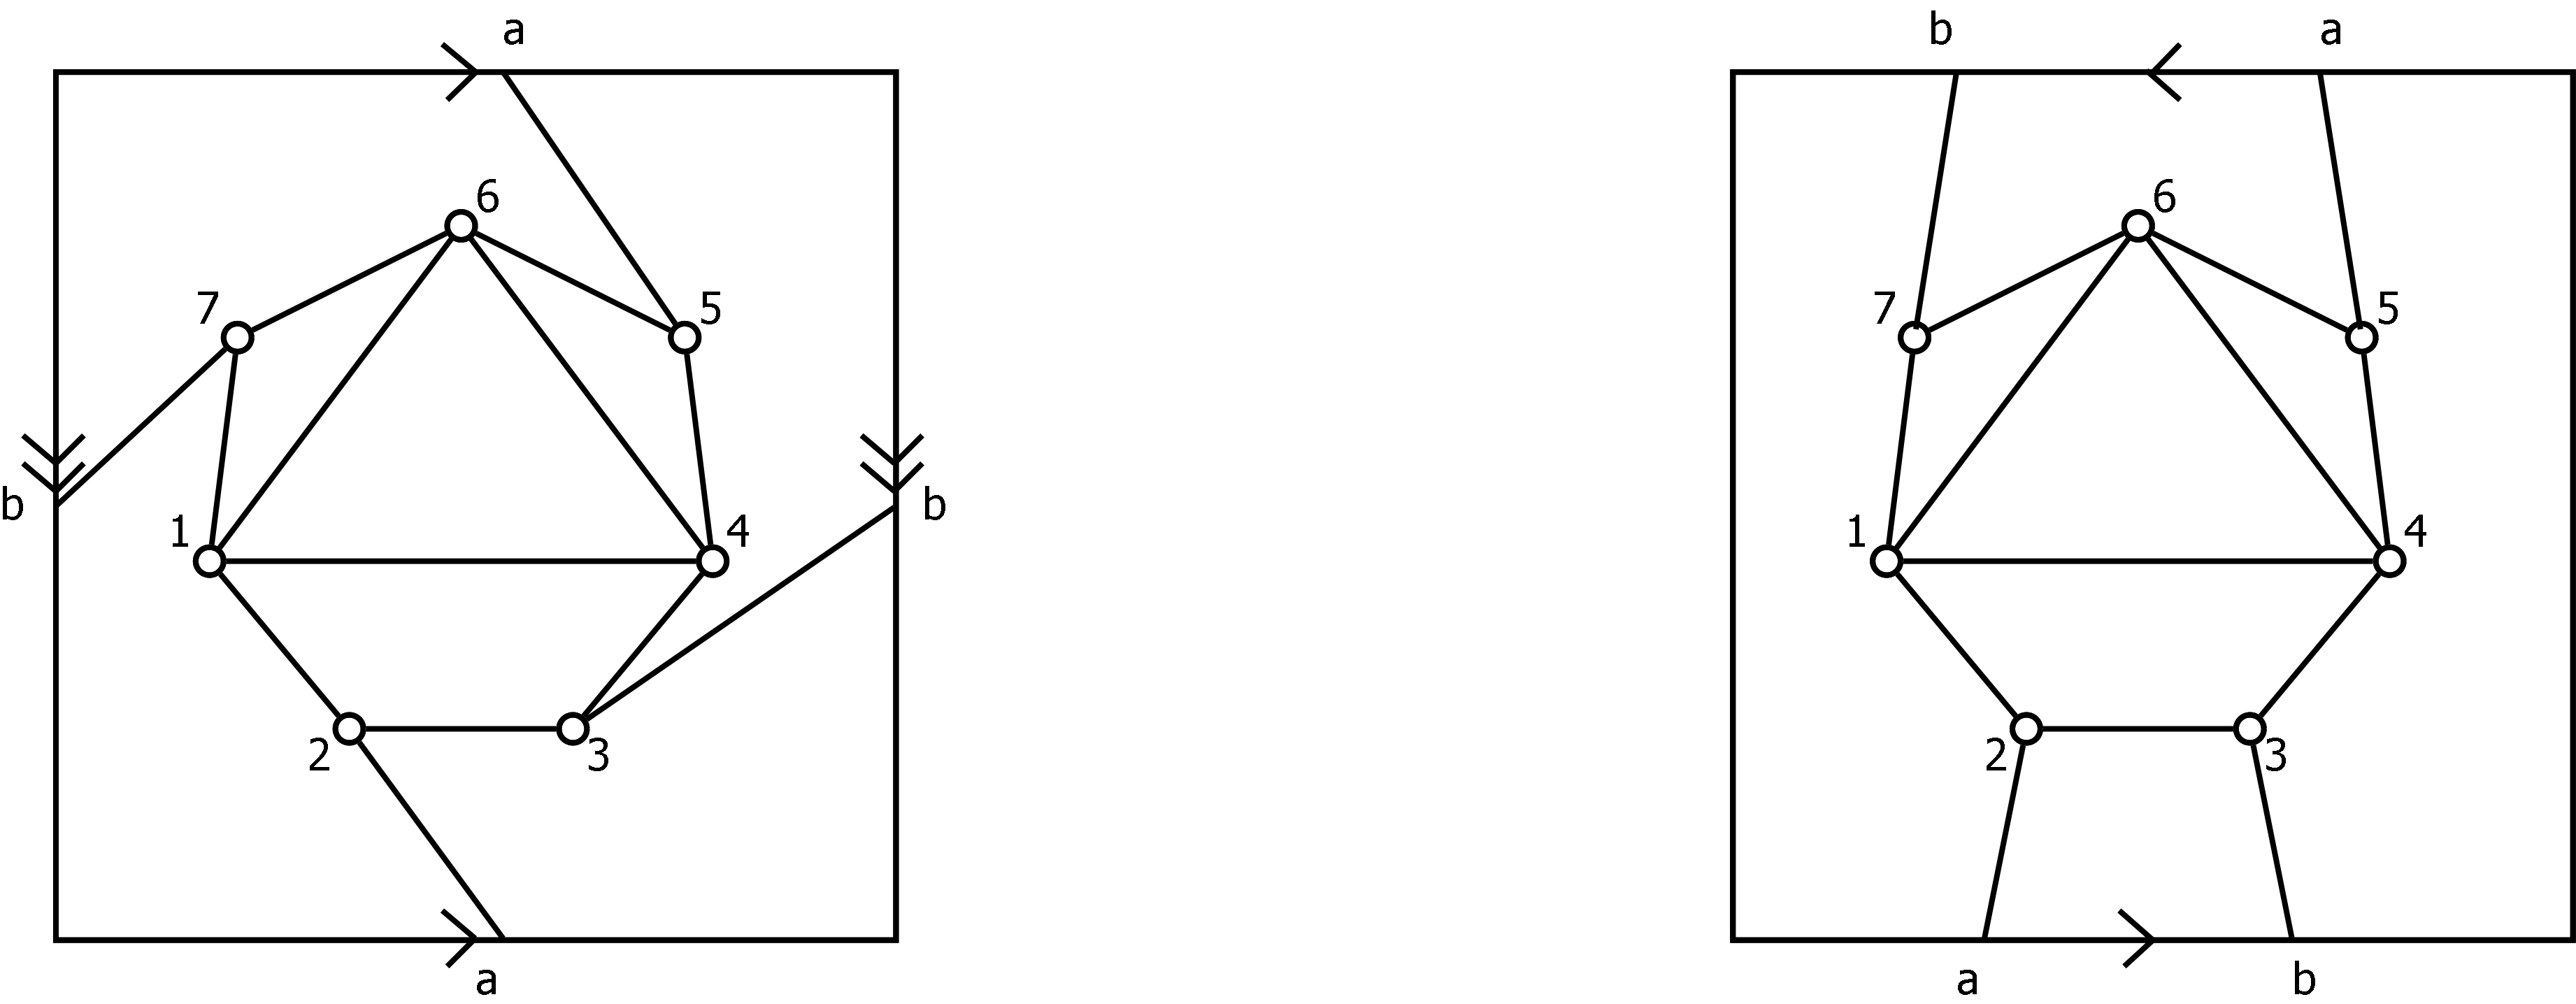
\includegraphics[width=\textwidth]{torusstrip35new.png}
\end{center}

Example 2:


To find a subgraph that's a subdivision of $K_{3,3}$, one way is the following@ take vertices 1, 11, and 13 to be the red vertices, and 3, 5, and 9 to the blue vertices.  Then 1 is adjacent to 5 and 9 in the graph, and we can connect it two 3 through vertex 4.  Vertex 13 is adjacent to 5 and 9 in the graph, and we can connect it to 3 through 13-14-7-3.  Finally, vertex 11 is adjacent to 3 in the graph.  We can connect it to 5 by 11-15-16-8-5, and to vertex 9 through vertex 12.

We haven't used any of the extra vertices more than once, so that is a subdivision of $K_{3,3}$.

To get a subdivision of $K_5$, we can take our vertices to be 1 and the 4 vertices adjacent to it, namely 2, 4,5 and 9.  By construction 1 is already connected to everything.  We can connect 2 to 5 through 3, connect 2 to 5 through 6, and connect 2 to 9 through 10.  WE can connect 4 to 5 through 8, and 4 to 9 through 12.  Finally, we can connect 5 to 9 through 13.








To draw it on the torus, we can do the following

\begin{center}
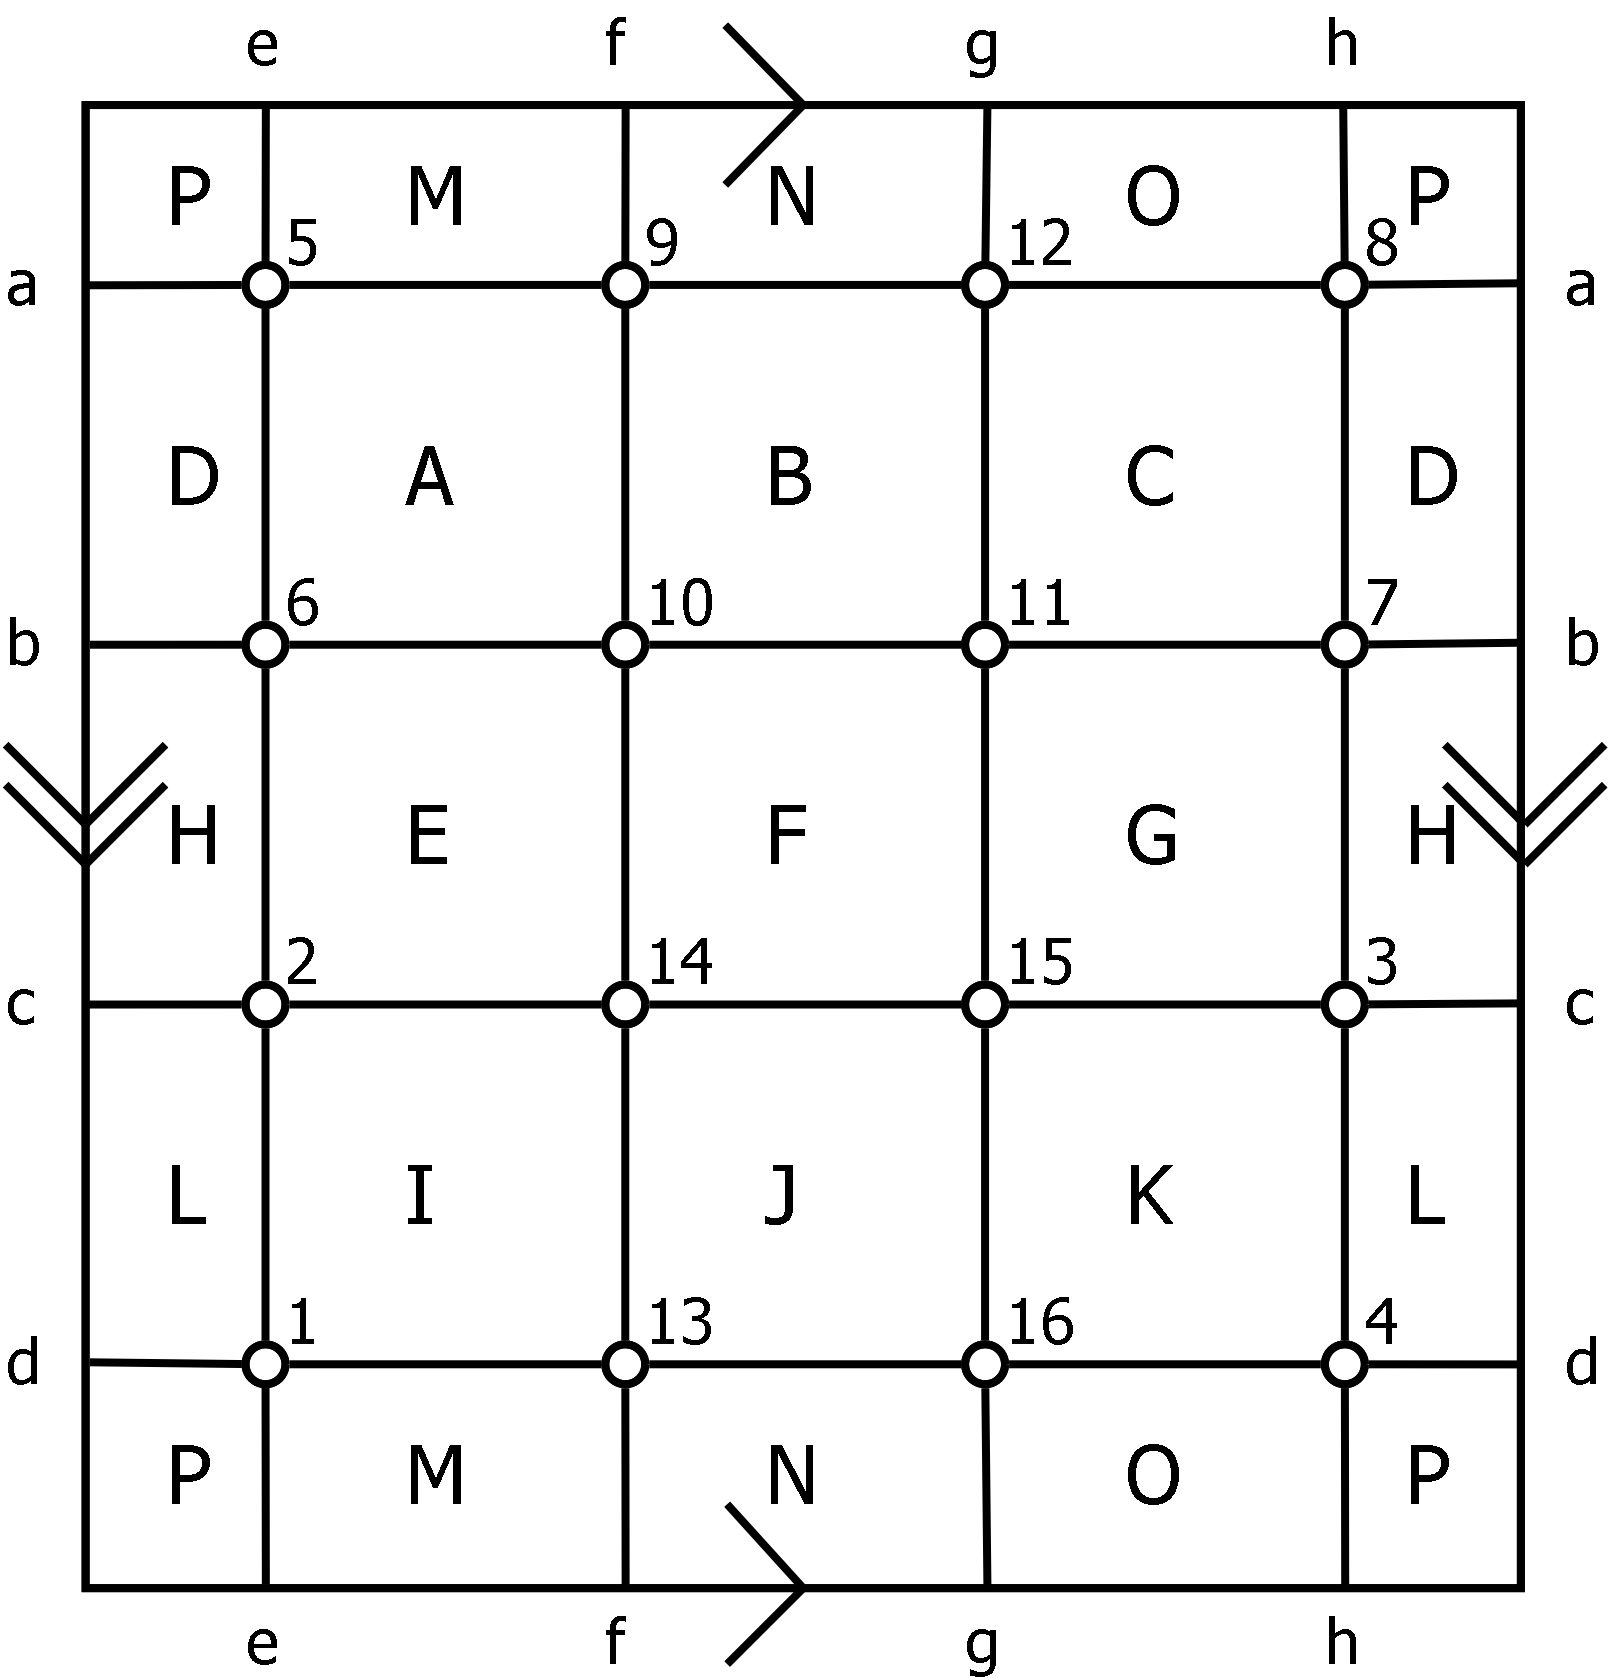
\includegraphics[width=\textwidth]{probbooksol36c.png}
\end{center}


\section{Week 8}

\subsection{Annoying to draw}

To draw the $K_{4,4}$ on the klein bottle, we can do the following:

\begin{center}
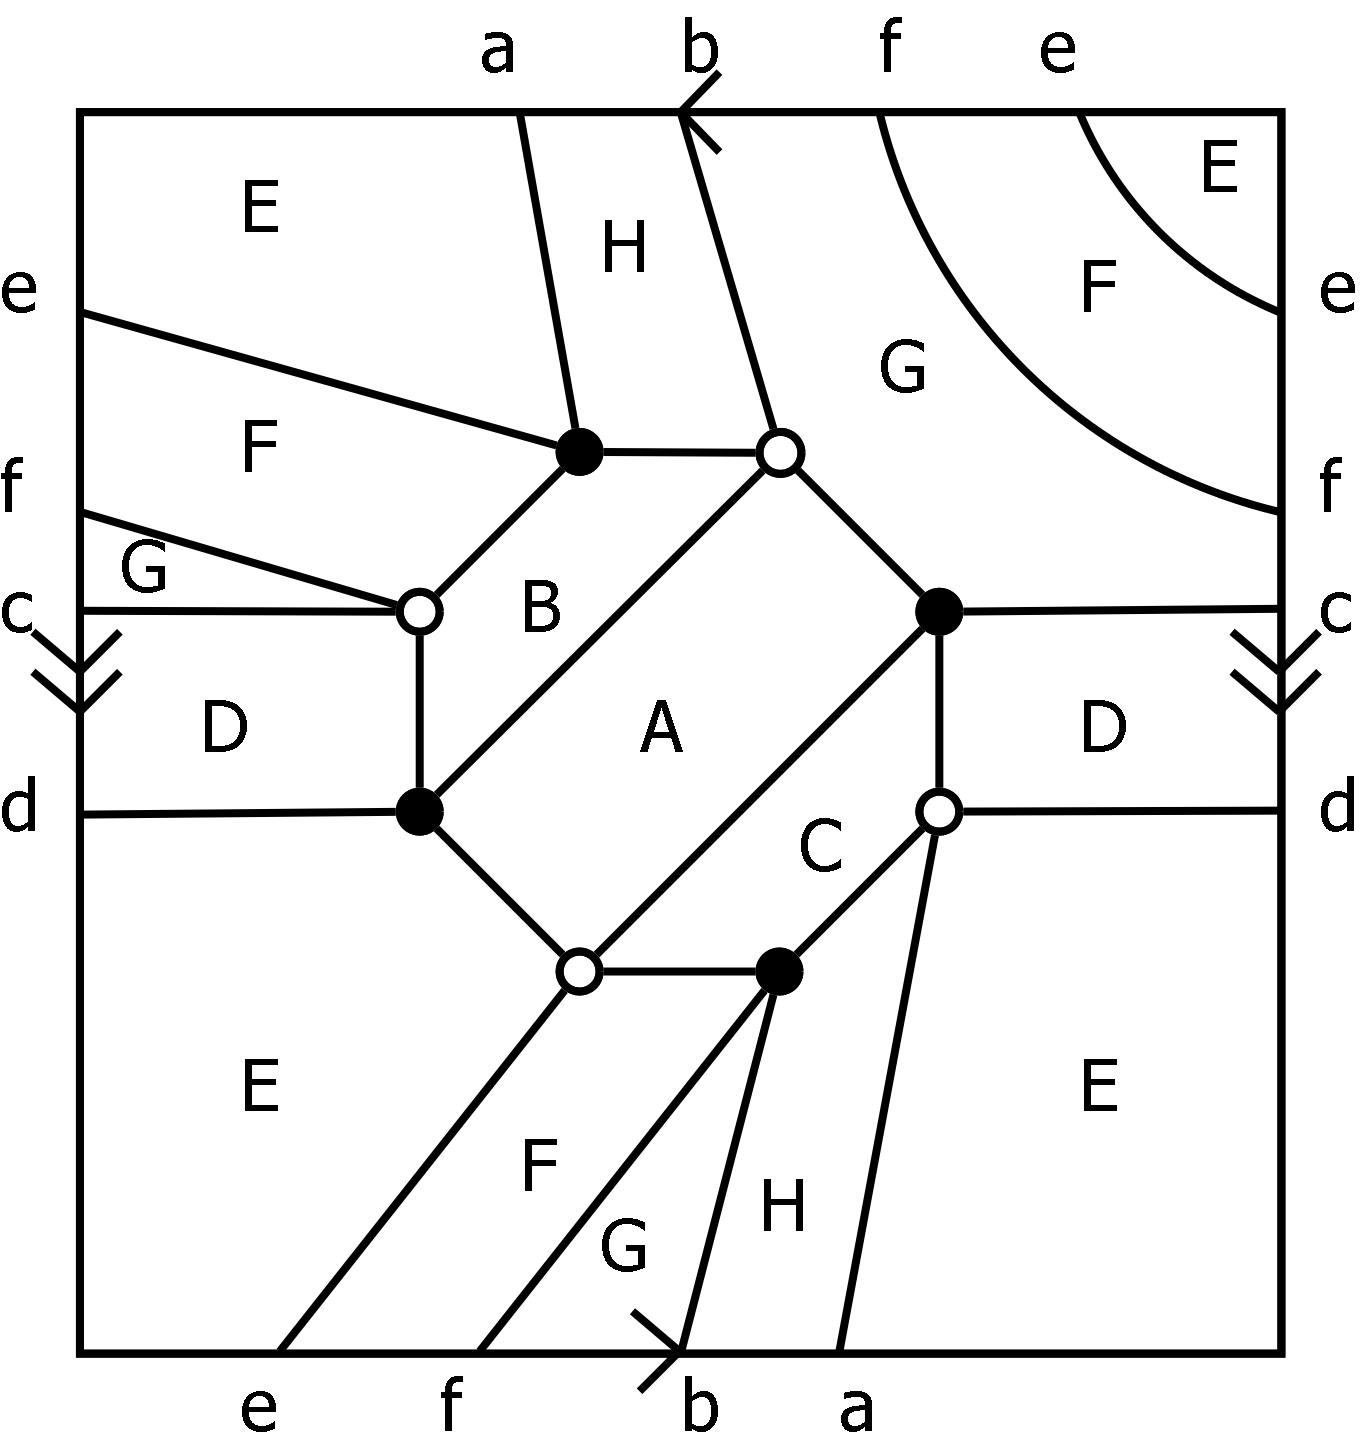
\includegraphics[width=\textwidth]{kleink-4-4.png}
\end{center}


\subsection{Proof 1}

TO prove that $K_{3,3}$ isn't planar using the handshaking lemma, note that $K_{3,3}$ has 6 vertices and 9 edges.  If we could draw it on the plane, then Euler's theorem $v-e+f=2$ becomes $6-9+f=2$, and so it would have five faces.

Now, we claim that each face would have to have at least 4 edges.  No face could have 1 edge since that would be a loop, and two edges would mean a multiple edge, and both of these aren't possible since $K_{3,3}$ is simple.  If a face had three edges, that would be a three cycle, but $K_{3,3}$ is bipartite and so has no three cycles.  Thus, any face must have at least 4 edges.

But then handshaking between faces and edges would give

$$18=2e=\sum_f d(f)\geq \sum_f 4=5*4=20$$
since we had 5 faces.  This is a contradiction, and so $K_{3,3}$ is not planar.

\subsection{Proof 2} 

  By handshaking, $2e=d_1v$ so $v=\frac{2e}{d_1}$. Similarly, using face-handshaking, $f=\frac{2e}{d_2}$. By Euler's formula,
\begin{align*}
e+2&=v+f \\
&=2e\left(\frac{1}{d_1}+\frac{1}{d_2}\right)
\end{align*}
so
\[
\frac{1}{d_1}+\frac{1}{d_2}=\frac{e+2}{2e}>\frac{1}{2}\,.
\]
If $d_1, d_2\geq 4$ then we would have $\frac{1}{d_1}+\frac{1}{d_2}\leq\frac{1}{4}+\frac{1}{4}=\frac{1}{2}$, a contradiction. So one of them must be 3, and then the other must be less than 6, since $\frac{1}{3}+\frac{1}{6}=\frac{1}{2}$. The possibilities are:

\begin{tabular}{|c|ccccc|}
\hline
$d_1$ & 3 & 3 & 3 & 4 & 5 \\
$d_2$ & 3 & 4 & 5 & 3 & 3 \\
example & tetrahedron & cube & dodecahedron & octahedron & icosahedron \\
\hline
\end{tabular}

\section{Week 9 Practice Problems}


\subsection{Chromatic number and chromatic index}

First, we do the 7 vertex graph. To find the chromatic number, suppose there is a colouring of the vertices with three colours. 1, 2 and 3 must all be different colours, say red, green and blue respectively. Now 4 is adjacent to 2 and 3, so must be red; 5 is adjacent to 3 and 4, so must be green; 6 is adjacent to 4 and 5 so must be blue; and 7 is adjacent to 5 and 6 so must be red. But this is not a valid colouring, since 7 and 1 are adjacent. So no colouring with three colours is possible. There is a 4-colouring, so $\chi(G)=4$.






Now, we find $\chi^\prime(G)$ for the 10 vertex graph.  Since there are only seven vertices, among any four edges some two will have a vertex in common. So no four edges can be the same colour in any edge-colouring. Suppose we have an edge colouring with 4 colours. Each colour is used on at most 3 edges, so there are at most 12 edges coloured. But $G$ has 14 edges, so another colour is required. It can be 5-edge-coloured, so $\chi'(G)=5$.

The following pictures illustrate the vertex and edge colourings.

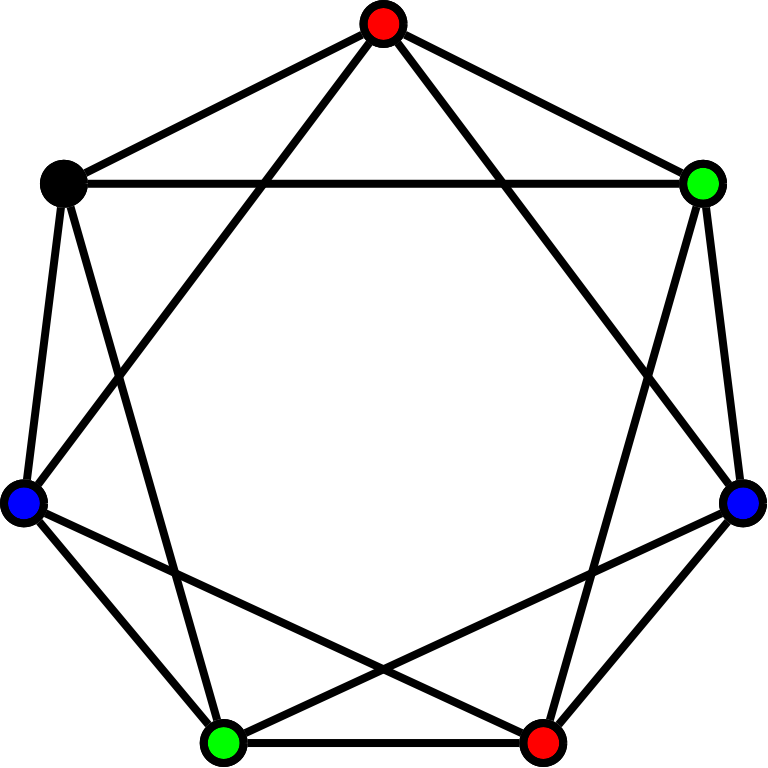
\includegraphics[width=.4\textwidth]{probbooksol53a.png}
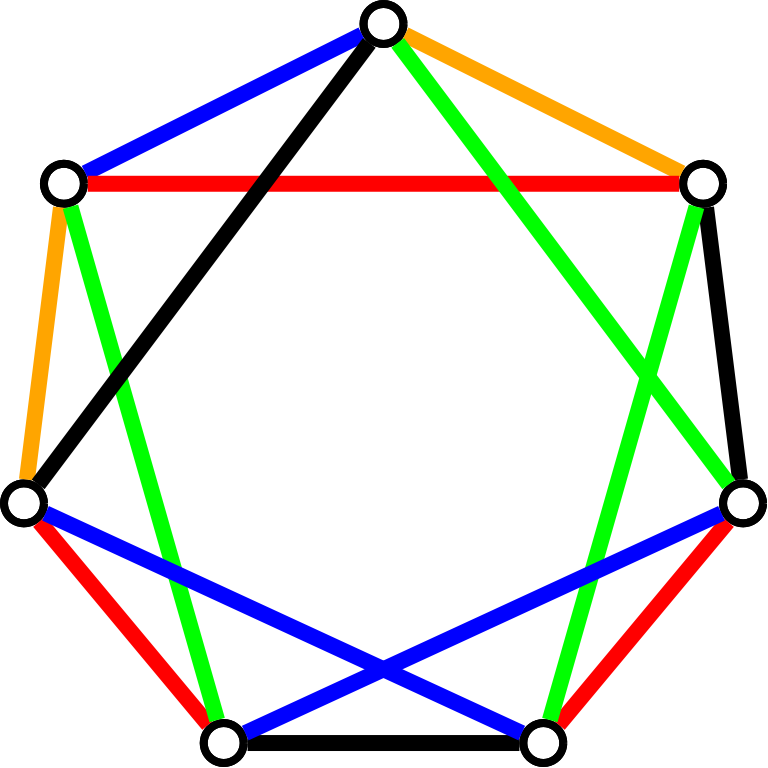
\includegraphics[width=.4\textwidth]{probbooksol53.png}




Now, we do the 10 vertex graph.  The graph contains $K_5$ as a subgraph, so its chromatic number is at least 5. A colouring with 5 colours exists, so $\chi(G)=5$.
\begin{center}
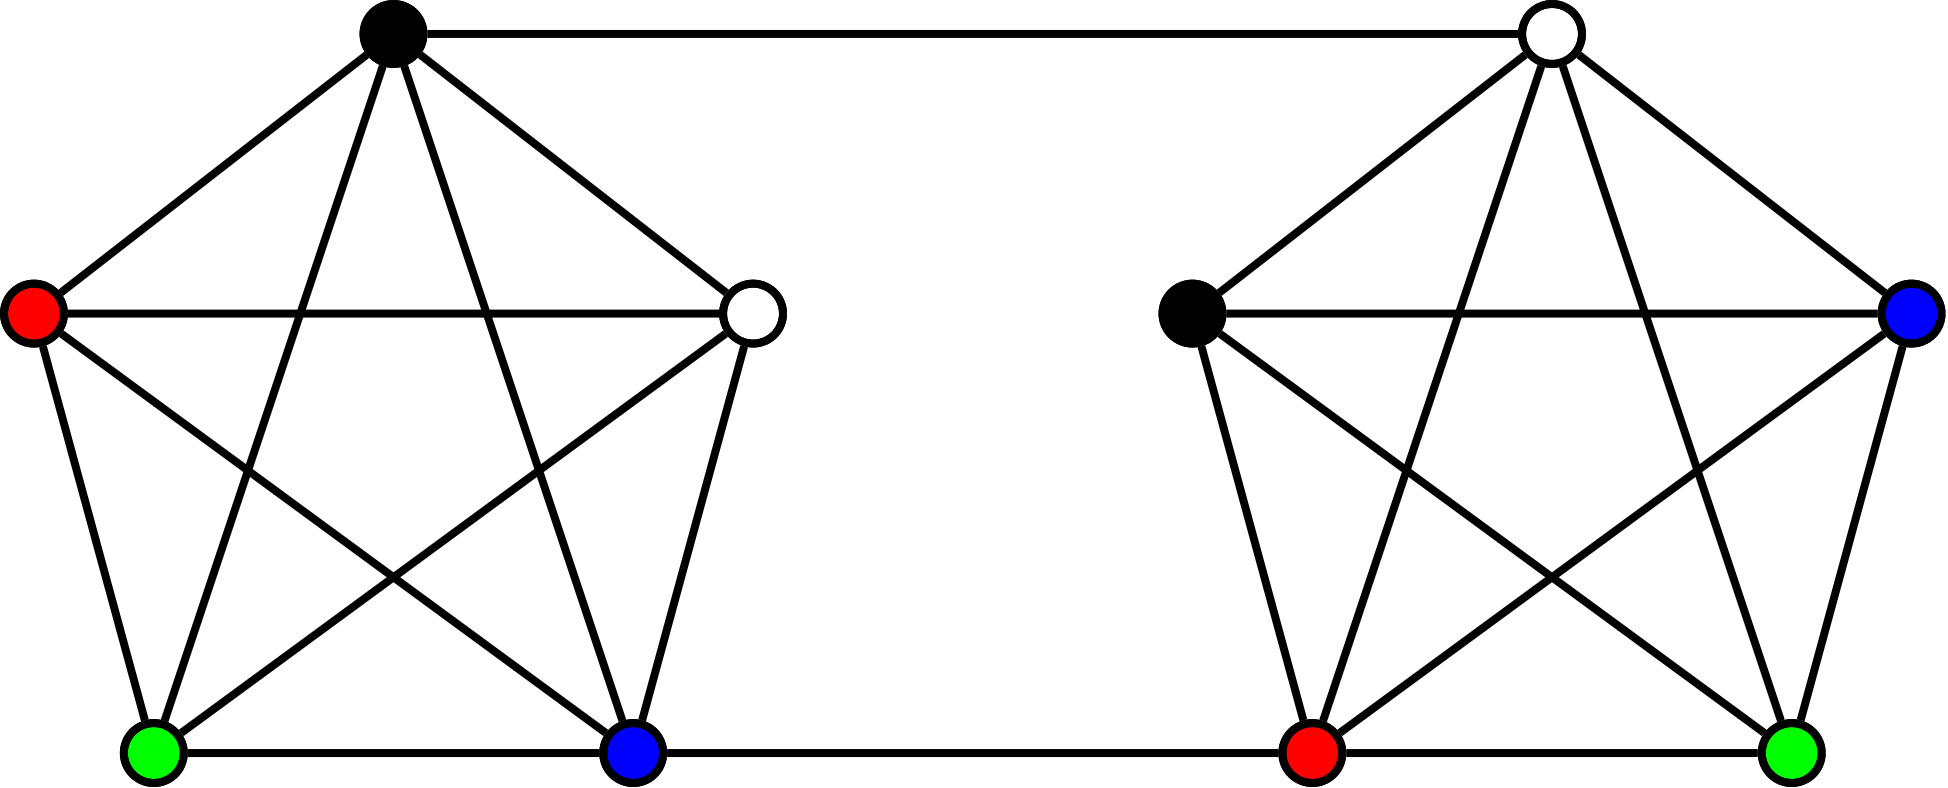
\includegraphics[width=.5\textwidth]{probbooksol51a.png}
\end{center}
$G$ has maximum degree 5, so $\chi'(G)\geqslant 5$. An edge colouring with 5 colours exists, so $\chi'(G)=5$.
\begin{center}
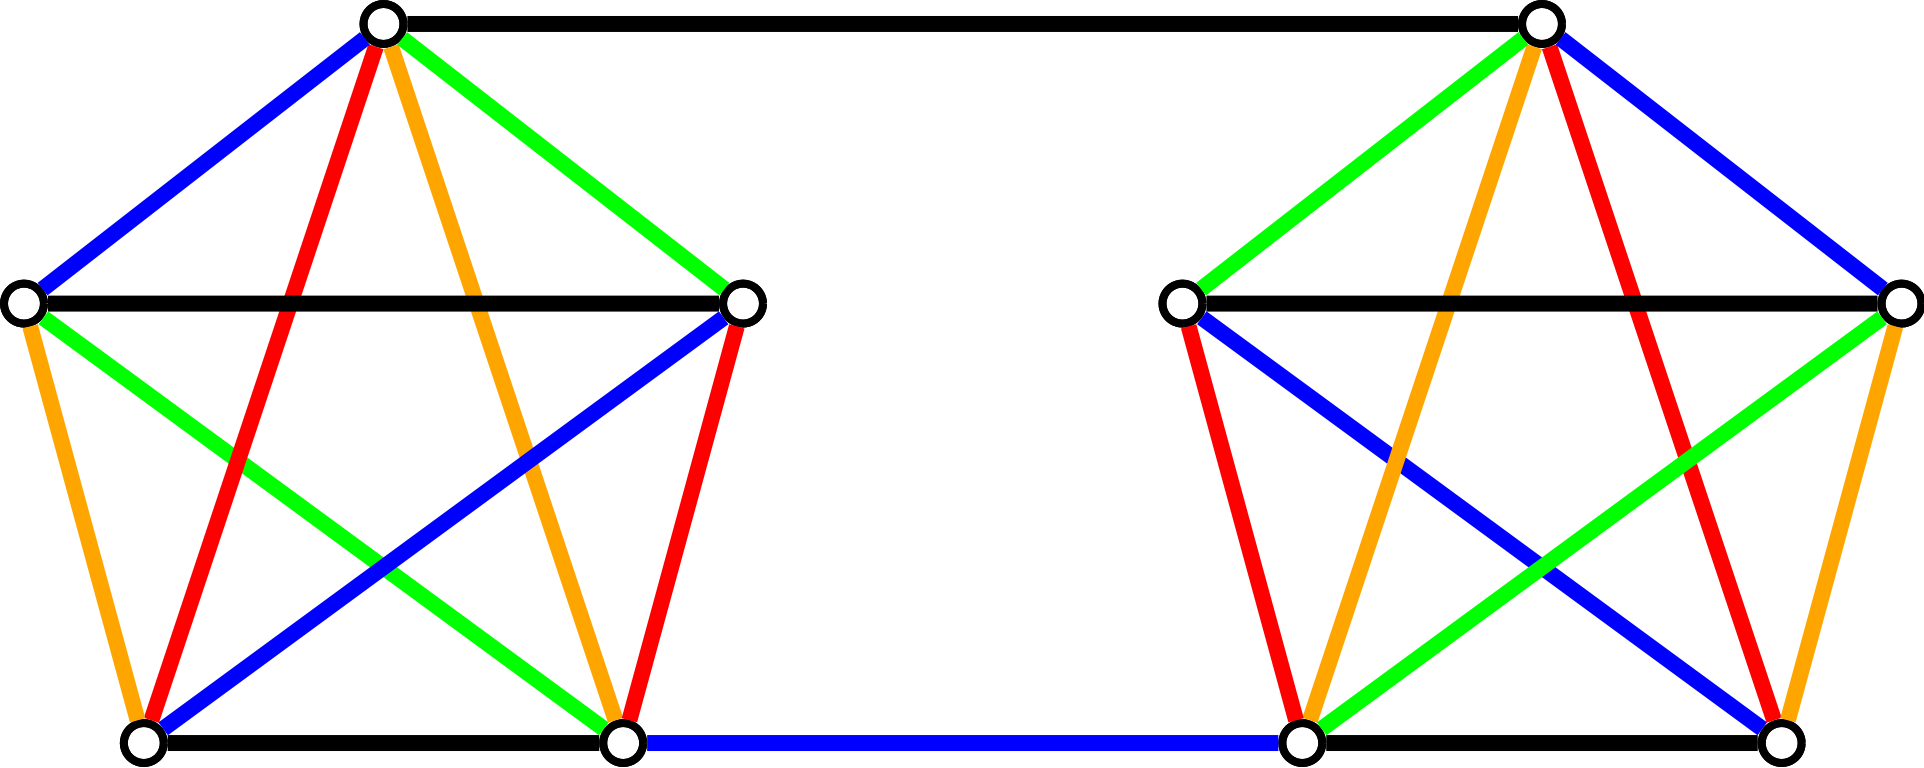
\includegraphics[width=.5\textwidth]{probbooksol51b.png}
\end{center}

\subsection{A word problem}
Draw a graph $M$ whose vertices are the teams and whose edges are the matches. An allocation of weeks to matches avoids clashes if and only if it is an edge colouring of the graph, so the minimum number of weeks is $\chi'(M)$.

We will show that $\chi'(M)>3$. Suppose we can colour the edges with red, green and blue. AH, HF and FA need three different colours, as each meets both of the others, so without loss of generality assume they are coloured red, green and blue respectively. Now AG must be green, HB must be blue, and FB must be red. Considering colours used at B, BE must be green. 

Now GD, DE and GE must be three different colours, but none of them can be green because each meets either AG or BE. So there is no edge colouring with three colours. An edge-colouring with four colours may be obtained by colouring GD red, DE blue, GE black and DC green, as shown, so $\chi'(M)=4$.

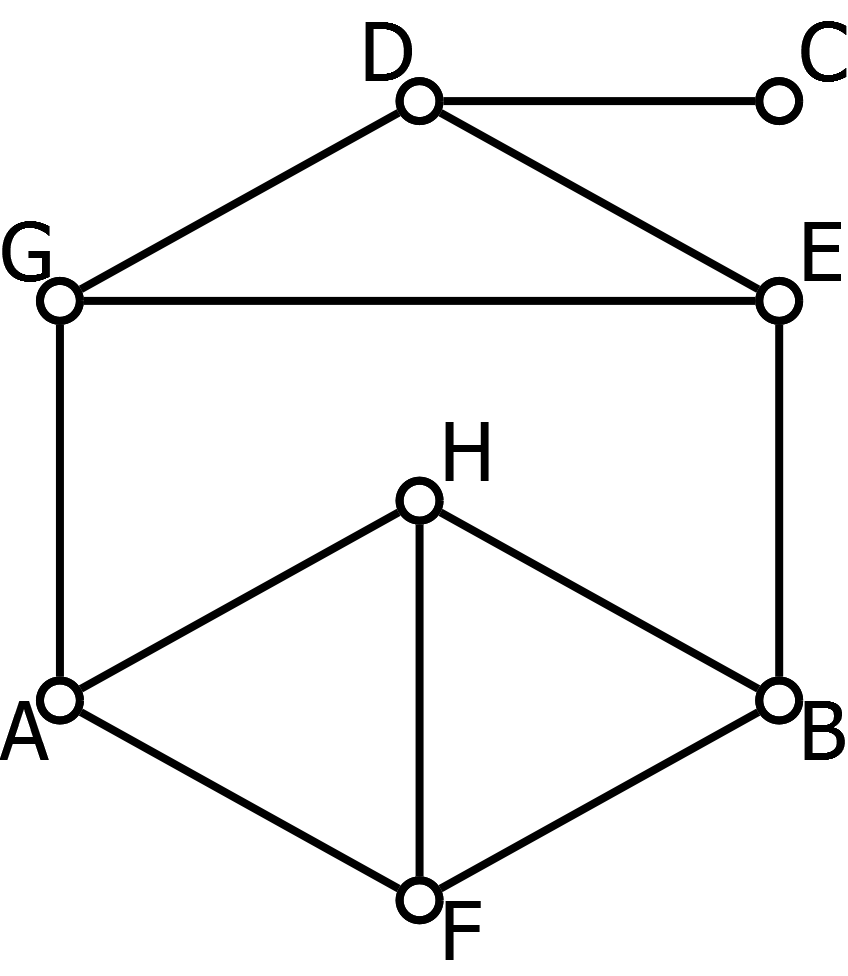
\includegraphics[width=.4\textwidth]{probbooksol44new.png}
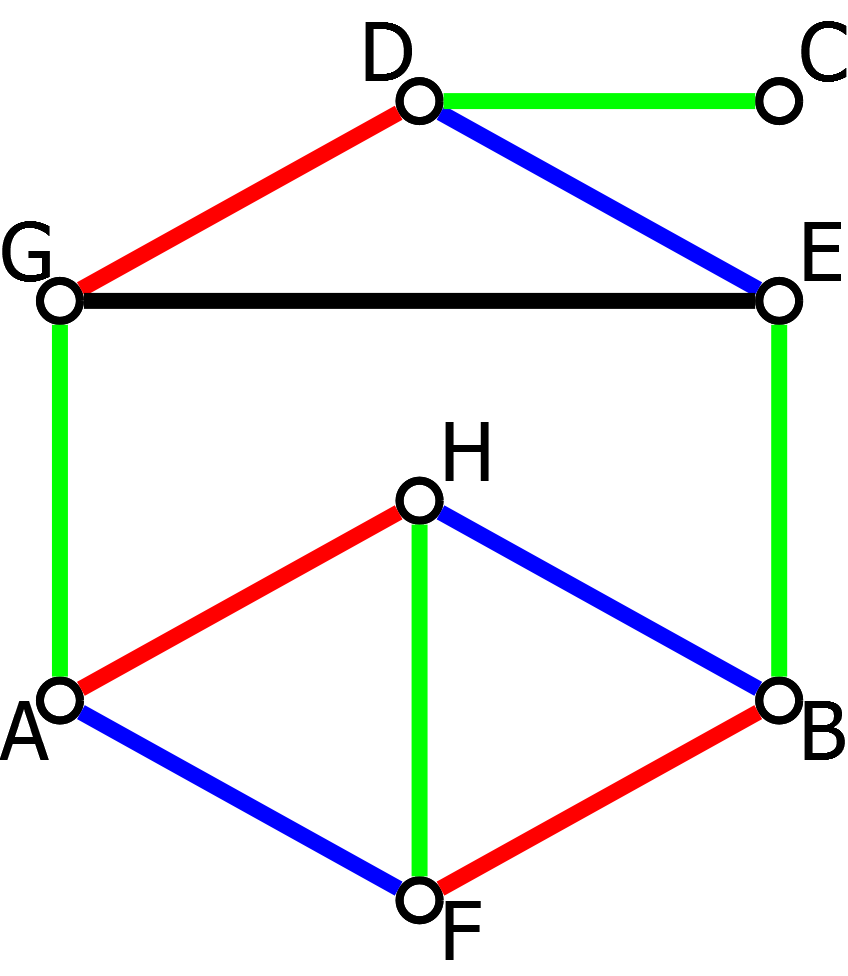
\includegraphics[width=.4\textwidth]{probbooksol44bnew.png}

\section{Week 10 Problems}

\subsection{Chromatic polynomials of cycles}

To find the chromatic polynomial of the 5 cycle, suppose we have labelled the vertices $1,2,3,4,5$ in cycle order.  Suppose we have a colouring of $C_5$ with $k$ colours; we begin by considering two cases: either vertex 1 and vertex 3 have the same colour, or they have different colours.

Case 1: If 1 and 3 have the same colour, there are $k$ ways to choose that colour. There are then $k-1$ ways to colour vertex 2, as it is adjacent to 1 and 3.  There are $k-1$ ways to colour vertex 4, as it is adjacent to 3, and then finally there are $k-2$ ways to colour vertex 5, as it is adjacent to vertex 1 and vertex 4, which we know have different colours.  Hence, case 1 gives $k(k-1)^2(k-2)$ possibilities.

Case 2: If 1 and 3 are different colours, there are $2$ ways to colour vertex 1, and then $k-1$ ways to colour 3.  There are then $k-2$ ways to colour vertex , as it is adjacent to both vertex 1 and 3, which have different colours.  There are $k-1$ ways to colour vertex 4, because it is adjacent to vertex 3, but now we have a problem, because vertex 5 is adjacent to vertex 1 and vertex 4, which may have the same colour, or may not.

There are a few ways around this difficulty.  One is to note that since vertex 1 and vertex 3 have different colours, this is the same as trying to colour the graph where we have added an edge between them.  This is the ``house graph'' -- a square and a triangle glued along the edge.  We know that there are $k(k-1)(k^2-3k+3$ ways to colour the square; when we go to colour the remaining vertex, it as adjacent to two vertices that have different colours, and so has $k-2$ possibilities, thus, there are $k(k-1)(k-2)(k^2-3k+3)$ possibilities for case II.

Adding case I and II together, we get:
$$k(k-1)^2(k-2)+k(k-1)(k-2)(k^2-3k+3)=k(k-1)(k-2)(k^2-2k+2)$$

Another approach is to change our two cases at the very beginning: consider vertices 1, 3 and 4.  In case A, they are all three different colours, while in Case B 1 is the same colour as either 3 or 4 (but not both, as 3 and 4 must have different colours.

Case A: There are $k(k-1)(k-2)$ ways to colour 1,3 and 4 so they all have different colours.  Now, there are $k-2$ ways to colour 2 and $k-2$ ways to colour 5, so there are $k(k-1)(k-2)^3$ ways total in case A.

Case B: There are two possibilities: 1 is the same colour as 3, and one is the same colour as 4, but they are clearly equivalent by a reflection of the graph.  Therefore, we just need consider the case where 1 is the same colour as 3, and multiply this by 2.  We saw that if 1 is the same colour as three, there are $k(k-1)^2(k-2)$ ways to colour the graph in whole, and so case B gives $2k(k-1)^2(k-2)$.

Adding Case A and Case B gives:
\begin{align*}
  k(k-1)(k-2)^3+2k(k-1)^2(k-2)&=k(k-1)(k-2)[k^2-4k+4+2(k-1)] \\
  &=k(k-1)(k-2)(k^2-2k+2)
  \end{align*}
so we've gotten the same answer.


\subsection{A series of examples}

To colour graph a, we know that that there are $k(k-1)(k^2-3k+3)$ ways to colour the central square.  There are then $(k-2)$ ways to colour each of the remaining vertices, giving $k(k-1)(k-2)^2(k^2-3k+3)$ as the number of ways to colour graph a.

To do Graph b, there are two methods.  The sneaky method is to first colour the one vertex of degree 4 in any of the $k$, which is adjacent to every other vertex.  It remains to colour a square, where none of the colours can be the same as the first vertex we coloured.  This means we are colouring the square with $k-1$ colours, which by definition is $\chi_{C_4}(k-1)$, which we get by replacing $k$ with $(k-1)$ in $k(k-1)(k^2-3k+3)$, giving $(k-1)(k-2)(k^2-5k+5)$, and so we see $\chi_{G_b}(k)=k(k-1)(k-2)(k^2-5k+7)$.

Graph b can also be done using deletion contraction on one of the edges $e$ of the square.  If we delete $e$, the resulting graph is three triangles joined along successive edges in a line, and it is easily seen that $\chi_{G_b\setminus e}(k)=k(k-1)(k-2)^3$.  If we contract $e$, we again have three triangles, but now they share a central vertex, which is easily seen to have $\chi_{G_b/e}(k)=k(k-1)(k-2)(k-3)$ in fact, this graph is $K_4$, so we knew that already.

Thus, by deletion contraction we have:
\begin{align*}
  \chi_{G_b}(k)&=\chi_{G_b\setminus e}(k)-\chi_{G_b/e}(k) \\
  &=k(k-1)(k-2)(k^2-4k+4)-k(k-1)(k-2)(k-3) \\
  &=k(k-1)(k-2)(k^2-5k+7)
\end{align*}



Finally, to do graph $c$, let $e$ the long edge from the far left vertex to the far right vertex.  One sees that $G_c/e=G_b$, while $G_c\setminus e=G_a$, and so deletion contraction gives

\begin{align*}
  \chi_{G_c}(k) &=\chi_{G_a}(k)-\chi_{G_b}(k) \\
  &=k(k-1)(k-2)^2(k^2-3k+3) -k(k-1)(k-2)(k^2-5k+7) \\
  &=k(k-1)(k-2)[k^3-5k^2+9k-6-(k^2-5k+7)] \\
  &=k(k-1)(k-2)[k^3-6k^2+14k-13]
\end{align*}


\end{document}
